\documentclass[12pt]{article}
\usepackage[top=1in,bottom=1in,left=1in,right=1in]{geometry}
\usepackage{alltt}
\usepackage{array}	
\usepackage{graphicx}
\usepackage{tabularx}
\usepackage{verbatim}
\usepackage{setspace}
\usepackage{listings}
\usepackage{amssymb,amsmath, amsthm}

\title{SOEN331: Introduction to Formal Methods\\for Software Engineering\\
Assignment 1 on extended finite state machines}
\author{Author's name}
\date{\today}

\begin{document}
\begin{spacing}{1.5}

\maketitle

\section{Washing Machine formal specification}

\noindent The EFSM of the washing machine is the tuple $S = (Q, \Sigma_1, \Sigma_2, q_0, V, \Lambda)$, where\\

\noindent $Q = \{off, on\}$\\
\noindent $\Sigma_1 = \{powerOn, powerOff\}$\\
\noindent $\Sigma_2 = \{beep;lightOff\}$\\
\noindent $q_0: off$\\
\noindent $V: \{\}$\\
\noindent $\Lambda$: Transition specifications\\
\indent 1. $\rightarrow off$\\
\indent 2. $off \xrightarrow {\text { powerOn }} on$\\
\indent 3. $on \xrightarrow {\text { powerOff / beep; lightOff}} off$\\
\newpage

\noindent As $on$ is a composite state, it is defined as the tuple $S = (Q, \Sigma_1, \Sigma_2, q_0, V, \Lambda)$, where\\

\noindent $Q = \{operating, service\}$\\
\noindent $\Sigma_1 = \{service [idle], serviceDone\}$\\
\noindent $\Sigma_2 = \{10secBlink;longBeep\}$\\
\noindent $q_0: operating$\\
\noindent $V: \{\}$\\
\noindent $\Lambda$: Transition specifications\\
\indent 1. $\xrightarrow {\text { /10secBlink;longBeep }} operating$\\
\indent 2. $operating \xrightarrow {\text { service [idle] }} service$\\
\indent 3. $service \xrightarrow {\text { serviceDone }} operating$\\

\noindent As $operating$ is a composite state, it is defined as the tuple $S = (Q, \Sigma_1, \Sigma_2, q_0, V, \Lambda)$, where\\

\noindent $Q = \{idle, standby, active\}$\\
\noindent $\Sigma_1 = \{start-finish, cancel [setting], cancel, powerLost, regainPower\}$\\
\noindent $\Sigma_2 = \{lightOn, unlock, clearSettings\}$\\
\noindent $q_0: idle$\\
\noindent $V: \{\}$\\
\noindent $\Lambda$: Transition specifications\\
\indent 1. $\xrightarrow {\text { /lightOn }} idle$\\
\indent 2. $idle \xrightarrow {\text { start-finish }} active$\\
\indent 3. $active \xrightarrow {\text { cancel }} idle$\\
\indent 4. $active \xrightarrow {\text { /unlock }} idle$\\
\indent 5. $active \xrightarrow {\text { cancel [setting] / clearSettings }} idle$\\
\indent 6. $active \xrightarrow {\text { powerLost }} standby$\\
\indent 7. $standby \xrightarrow {\text { regainPower }} active$\\


\noindent The UML state diagram is shown in Figure~\ref{fig:wm-fig}.\\\\

%MISSING ACTIVE COMPOSITE STATE
\newpage

\section{UML state diagrams}

\begin{figure}[h!]
	\centering
		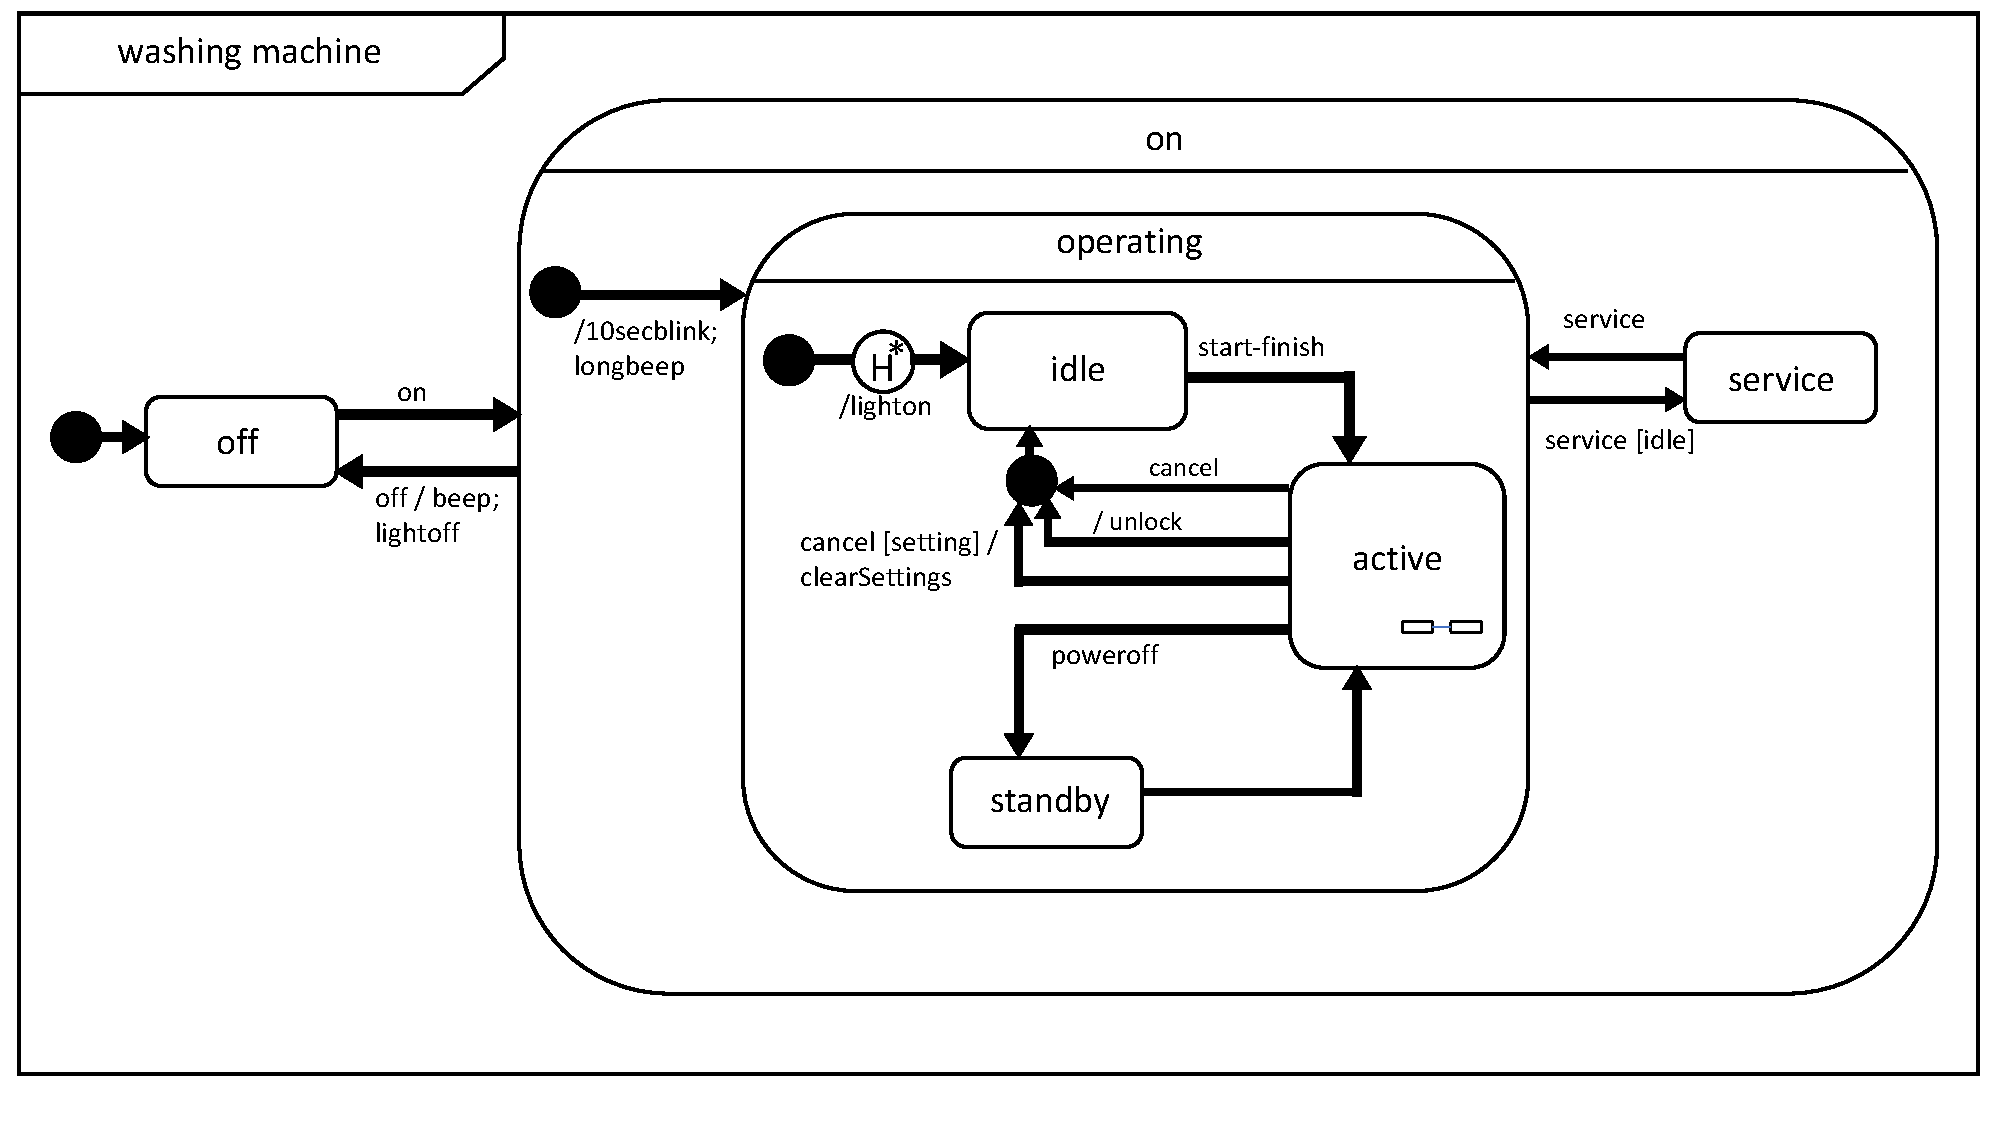
\includegraphics[width=0.8\textwidth]{./figures/a3-diagram-draft.pdf}
		  \caption{Washing Machine.}
  \label{fig:wm-fig}
\end{figure}

\end{spacing}
\end{document}
